\documentclass[a4paper, 10pt]{article}
\usepackage[UTF8]{ctex}
\usepackage{geometry}
\geometry{left=3cm,right=3cm,top=3cm,bottom=3cm}
\usepackage{subfigure}
\usepackage[graphicx]{realboxes}
\begin{document}
  \title{实验报告:金属杨氏模量的测量}
  \author{郑志恒 2300012559}
  \maketitle
  \section{CCD成像法测量金属丝的杨氏模量}
  \subsection{实验设备}
  \noindent \textbf{测定杨氏模量专用支架:}支架和金属丝,金属丝下端连接一小圆柱,圆柱中部方形窗中有细横丝供读数用;

  \vspace{10pt}
  \noindent \textbf{显微镜:}总放大率 25 倍,目镜距10mm,目镜前分划板刻度范围0至6.5nm,分度值0.05mm,允差0.005mm;每隔1mm刻一数字;
  
  \vspace{10pt}
  \noindent \textbf{CCD成像系统:}CCD摄像机,监视器;
  
  \vspace{10pt}
\noindent 米尺:带有卡口,分度值:1mm,允差:0.15mm

\noindent 螺旋测径器:量程:0~25mm,分度值:0.01mm,允差:0.004mm

\noindent 电子天平:分度值0.01g,允差:0.02g

\subsection{实验原理}
\noindent 根据胡克定理,材料在弹性限度内,正应力的大小$\sigma$与应变$\epsilon$成正比,即
$$\sigma=E\epsilon$$
$E$称为弹性模量,又称杨氏模量,其单位为Pa。对于长为$L$、截面积为$S$的均匀金属丝或棒,在沿长度方向的外力$F$作用下伸长$\delta L$,有$\sigma=F/S=\delta L/L$,则有
$$E=\frac{FL}{S\delta L}$$
利用此式测定杨氏模量的方法称为伸长法,
\subsection{实验过程}
\noindent \textbf{1.调节仪器}

\noindent i.调支架铅直,调小圆柱两侧小螺丝,限制小圆柱转动,并使金属丝下端的小圆柱与钳形平台间无摩擦地上下移动。

\noindent ii.先调显微镜目镜,用眼睛看到清晰的分划板像,再调物镜对小圆柱中部方形窗内细横刻线聚焦。

\noindent iii.连接CCD和监视器,打开监视器,仔细调节CCD位置及镜头光圈的焦距,直到在监视器屏幕上看到清晰的像。

\vspace{10pt}
\noindent \textbf{2.观测金属丝受外力拉伸后的伸长变化}

\noindent 称量9个砝码的质量。在砝码托盘上逐次加砝码,金属丝伸长后,对应的读数r(i=0,1,2,...,8,9).再将所加砝码逐个减去,记下对应的读数r'(i=0,1,2,...,8,9)

\vspace{10pt}
\noindent \textbf{3.测量金属丝L(一次测量)和金属丝直径d(测10次)}

\noindent 用米尺测量金属丝可伸长部分(两固定点之间)的长度,用螺旋测微器测量金属丝不同位置的直径,测量10次。


\subsection{数据记录}

\vspace{10pt}
\begin{center}
    \begin{tabular}{|c|c|c|c|c|c|}
      \hline
      $i $& $m_i/g$ & $r_{i1}/mm$ & $r_{i2}/mm$ & $\overline{r}$/mm&$\delta L$/mm\\
      \hline
      0 &0 &2.33&2.33&2.33&/\\
      \hline
      1 & 199.52&2.47&2.50&2.485&/\\
      \hline
      2 &399.30 &2.62&2.64&2.63&/\\
      \hline
      3 & 599.17&2.75&2.77&2.76&/\\
      \hline
      4 &799.16 &2.87&2.89&2.88&/\\
      \hline
      5 &999.12 &3.00&3.03&3.015&0.775\\
      \hline
      6 &1198.92 &3.11&3.13&3.12&0.635\\
      \hline
      7 & 1398.84&3.25&3.26&3.255&0.625\\
      \hline
      8 &1598.57 &3.36&3.37&3.365&0.605\\
      \hline
      9 & 1798.46&3.50&3.50&3.50&0.620\\
      \hline
    \end{tabular}
  \end{center}
\subsubsection{逐差法处理数据}
\noindent (因为不同砝码的质量略有不同,因此这里使用逐差法先求出每一个$\delta L$对应的$\delta L/\Delta m$,再求平均)利用上表的$\delta L$算出$\frac{\Delta L}{\Delta m}$的平均值有
$$\frac{\Delta L}{\Delta m}=0.00064298mm/g$$
测量十次金属丝直径有:
\begin{center}
    \begin{tabular}{|c|c|c|c|c|c|c|c|c|c|c|}
      \hline
      $i $& 1 & 2 & 3 & 4&5&6&7&8&9&10\\
      \hline
      d(cm)&0.033 &0.032 &0.032&0.032&0.032&0.033&0.032&0.032&0.032&0.032\\
      \hline
      
    \end{tabular}
  \end{center}

\noindent 得到金属丝直径$d=0.032cm$,单次测量得到金属丝长度为$L=78.1cm$,代入公式计算得到:
$$E=\frac{4\delta mgL}{\pi d^2\delta L}=1.48\times 10^{11}Pa$$

\vspace{10pt}
\noindent \textbf{不确定度分析:}
$$\sigma_{re}=0.005/\sqrt{3}mm$$
逐差法得到系统误差有:
$$\sigma_{\delta La}=\sqrt{\frac{\sum_{i=1}^5(\delta L-\delta \overline{L})^2}{5\times 4}}=0.031mm$$
故有:
$$\sigma_{\delta L}=\sqrt{\sigma_{La}^2+2\sigma_{re}^2}=0.031mm$$
$$\sigma_{\delta m}=\sqrt{2}\times0.02g/\sqrt{3}$$
$$\sigma_d=\sqrt{(0.1\times\sqrt{\frac{\sum_{i=1}^{10}(d-\overline{d})^2}{10\times 9}})^2+(\sigma_{de}/\sqrt{3})^2}=0.0023mm$$
$$\sigma_L=1/\sqrt{3}mm$$
故有总的不确定度:
$$\sigma_E=4.3\times10^9Pa$$
综上逐差法处理结果为:
$$E=(1.48\pm 0.043)\times10^{11}Pa$$
\subsubsection{最小二乘法处理数据}
\noindent 得到$\Delta L$-$\Delta m$直线有:

\vspace{10pt}
\begin{figure}[ht]
    \centering 
    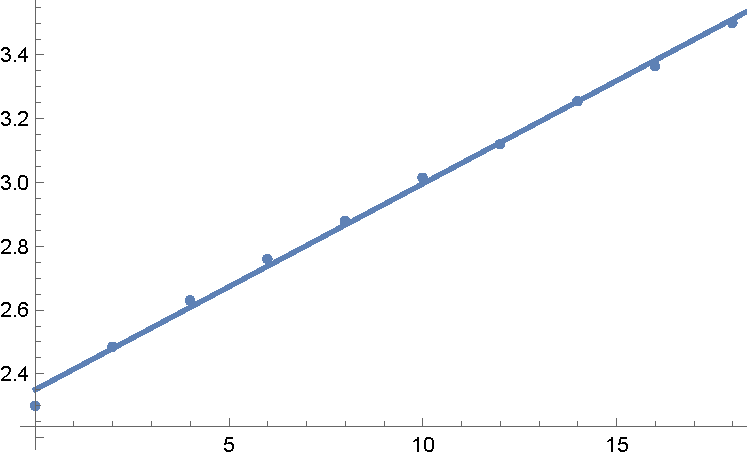
\includegraphics[height=9cm,width=13.5cm]{fg.pdf}
    
    \caption{fig1}
    \label{1}
    
    \end{figure}

\noindent 斜率的计算:
$$k=\frac{\sum_{i=1}^{10}(x_i-\overline{x})(y_i-\overline{y})}{\sum_{i=1}^{10}(x_i-\overline{x})^2}=0.064(mm/kg),r=0.998333$$
斜率的不确定度:
$$\sigma_{k}=\sqrt{(k\times\sqrt{\frac{1/r^2-1}{8}})^2+(0.005/\sqrt{3})^2}=0.0032mm/kg$$
其它不确定度同前,故有总的不确定度:
$$\sigma_E=7.7\times 10^9Pa$$
综上,最小二乘法的处理结果为:
$$E=(1.48\pm 0.077)\times10^{11}Pa$$
\section{光杠杆法测杨氏模量}
\subsection{实验过程}

\noindent \textbf{i.‌调整光杠杆系统‌:}

\noindent 将光杠杆后足尖放在夹紧钢丝的夹具的小圆平台上,以确保钢丝因受力伸长时,光杠杆平面镜倾斜;调整望远镜,调节目镜,使叉丝位于目镜的焦平面上,调整望远镜上下、左右、前后及物镜焦距,直到在望远镜中能看到清晰的直尺像。

\vspace{10pt}
\noindent \textbf{ii.‌加砝码和记录数据‌:}

\noindent 在钢丝下逐个加砝码,每加一个砝码,记下相应的直尺刻度值。再逐个减砝码,每减一个砝码,记下相应的直尺刻度值。

\vspace{10pt}
\noindent \textbf{测量其它数据:}

\noindent 根据原理公式,还需要测量金属丝长度L,光杠杆系统到平面镜距离R,光杠杆系统的径向长度D,金属丝的直径d

\subsection{数据处理}
\noindent 原理公式:
$$E=\frac{8FLR}{\pi d^2D \delta L}$$
实验数据如下:
\begin{center}
    \begin{tabular}{|c|c|c|c|c|}
      \hline
      $i $& $m_i/g$ & $r_{i1}/cm$ & $r_{i2}/cm$ & $\overline{r}$/cm\\
      \hline
      0 &0 &4.32&4.30&4.31\\
      \hline
      1 & 199.52&3.98&4.00&3.99\\
      \hline
      2 &399.30 &3.66&3.65&3.655\\
      \hline
      3 & 599.17&3.38&3.35&3.565\\
      \hline
      4 &799.16 &3.06&3.00&3.03\\
      \hline
      5 &999.12 &2.70&2.65&2.68\\
      \hline
      6 &1198.92 &2.35&2.35&2.35\\
      \hline
      7 & 1398.84&2.04&2.02&2.03\\
      \hline
      8 &1598.57 &1.72&1.74&1.73\\
      \hline
      9 & 1798.46&1.39&1.39&1.39\\
      \hline
    \end{tabular}
  \end{center}
  \noindent 得到
  $$\overline{(\delta L/F)}=0.001657m/N$$

\noindent 测得其它数据有:
$$L=78.1cm$$
$$R=139.5cm$$
$$D=9.5cm$$
$$d=0.032cm$$
根据公式有:
$$E=1.72\times 10^{11}Pa$$
\section{梁的弯曲测杨氏模量}
\subsection{实验过程}
\noindent i.将待测金属梁放置在两个刀刃上,并在梁的中点悬挂砝码,记录梁的弯曲程度。

\vspace{10pt}
\noindent ii.使用读数显微镜测量微小位移,逐渐增加砝码,记录每次增加砝码后梁的弯曲情况‌。

\vspace{10pt}
\noindent iii.测量其它数据:根据原理公式,还需要测量梁的长度l、厚度h和宽度a
 \subsection{数据处理}

\noindent 原理公式:
 $$E=\frac{Gl^3}{4\lambda a h^3}$$

\noindent 实验数据如下:
\begin{center}
    \begin{tabular}{|c|c|c|}
      \hline
      $i $& $m_i/g$ & $s(mm)$ \\
      \hline
      0 &0 &32.5\\
      \hline
      1 & 199.52&32.0\\
      \hline
      2 &399.30 &31.2\\
      \hline
      3 & 599.17&30.3\\
      \hline
      4 &799.16 &29.5\\
      \hline
      5 &999.12 &28.7\\
      \hline
      
      
    \end{tabular}
  \end{center}

  \noindent 得到
  $$\overline{(\lambda/G)}=0.000388m/N$$

\noindent 测得其他数据有:
$$l=21.3cm$$
$$a=1.20cm$$
$$h=1.35mm$$
\noindent 得到杨氏模量的计算结果:
$$E=2.10\times 10^{11}Pa$$

\section{分析与讨论}
\noindent \textbf{i.开始加第一、二个砝码的时候r的变化量较大}

\noindent 第一,这可能因为金属丝在自由下垂的时候自身存在一定弯曲,因此第一、二个砝码不仅由于拉伸作用使得金属丝长度增长了一部分,并且还将金属丝从弯曲的状态拉直了一些,因此此时测得的长度变化较大于后续长度的变化。第二,也可能是由于调节后金属丝上下未夹紧,增加砝码时金属丝有一定的下滑。

\vspace{10pt}

\noindent \textbf{i.开始加第一、二个砝码的时候r的变化量较小}


\noindent 这可能是因为金属丝与支架之间存在一定摩擦,在砝码较小的时候,这些摩擦造成的影响相对较大,导致金属丝拉伸的长度小于正常值。
\end{document}